%%%%%%%%%%%%%%%%%%%%%%%%%%%%%%%%%
% 6CCS3PRJ Final Year Individual Project Report
% jan_aldous.torres@kcl.ac.uk
%%%%%%%%%%%%%%%%%%%%%%%%%%%%%%%%%
\documentclass[11pt]{informatics-report}
\usepackage{color}
\usepackage[square,sort,comma,numbers]{natbib} %References
\usepackage{graphicx}
\graphicspath{ {images/} }
\usepackage{textcomp}

%%%%%%%%%%%%%%%%%%%%%%%%%%%%%%%%%
% Front Matter - project title, name, supervisor name and date
%%%%%%%%%%%%%%%%%%%%%%%%%%%%%%%%%
\title{Population visualization tool for Lambeth Council}
\author{Jan Aldous Torres}
\studentID{1323454}
\supervisor{Dr Simon Miles}

\date{\today}

\abstractFile{FrontMatter/abstract.tex}
\ackFile{FrontMatter/acknowledgements.tex} %Remove line if you do not want acknowledgements

\begin{document}
\createFrontMatter
\onehalfspacing
\tableofcontents
\listoffigures
\doublespacing

%%%%%%%%%%%%%%%%%%%%%%%%%%%%%%%%%
% Report Content
%%%%%%%%%%%%%%%%%%%%%%%%%%%%%%%%%
% You can write each chapter directly here or in a separate .tex file and use the include command.

\chapter{Introduction}
\cite{_developing_classification}
\cite{kent_midway}
\cite{boden_detecting_2013}
\cite{conway_data_2014}
\cite{customer_segmentaion}
\cite{graves_visualization_2013}
\cite{smart_cities}
\cite{acorn_user_guide}
\cite{gogolou_data_2016}
\cite{lga_guide}
\cite{experian}

Local government councils are challenged with the recent cuts in local government funding and a diverse population with different needs. Therefore, there is a need to efficiently allocate resources. The usual approach is to tackle issues raised by individual social services. However, there has been a shift in local government, which is promoted by the national government, to utilize the concept of customer segmentation. This will let them understand the needs of the population better thus letting them utilize and allocate resources in the most effective way based on those needs [4]. This approach would require the council to identify and therefore focus resources on vulnerable population groups. For example, instead of focusing on issues on education, they would focus on the children in care who are most susceptible to lower educational, social and employment outcomes. Some social services deal with the same population groups so this approach would require an integration of data from the different services. This gives an overview of all data from services provided by the councils. This is unlike the former approach which requires individual social services to conduct data analysis using their own data.[TJA1] \par

Lambeth Council in London wants to implement the new approach. However, current methods to analyze and visualize data take a long time before the analyses and visualizations would reach the commissioners, the people in the council who formulate strategies to tackle issues.\par
 
There are off-the-shelf software packages available which supports users in customer segmentation from clustering to the visualization of their data. In government, using data analysis in policy decision making is becoming more popular(new york guy video). The Local Government Agency has created a guideline to support councils in tailor-made clustering and visualization [4]. Moreover, there have been projects by other local councils to visualizations of data on prominent population groups. \par

Lambeth Council would like to have a bespoke population segmentation tool that would be customized to their own needs and available data. This project aims to implement a prototype of such a tool as a Django web application.\par

The tool will focus on the situation in which population groups are in through visualizations. The situations they face will be defined by the data. Visualizations of this data will also help to compare characteristics of the group to the wider population and subgroups. This comparison may lead to observations on which problems a group or subgroup is facing. This may lead to the conclusion that the council may want to increase resources spent on a group or service. The tool basically aid the commissioner to apply customer segmentation on their population and identify which problems segments of the population are facing thus help make decision on the allocation of their resources.\par

Clustering will provide a more complete perspective into the different situations groups face instead of viewing a group as one entity and defines variables which distinguish the group from the rest of the population using clustering algorithms. Data integration from open government datasets will create a more in depth view of groups. And possible relations between geographical locations’ characteristics ie facilities (GP), situation (crime) in a ward and whether they are on the London living wage. Since the user may not necessarily know what they are looking for when they read the data, the visualizations will be in the form that will let the user explore more aspects of the data.\par

\section{Report Structure}
The remainder of this paper is organized as follows. Chapter 2 introduces related work to the tool and data exploration, and Chapter 3 discusses the requirements of the tool. Chapter 4 outlines the specification and design of the tool. Chapter 5

\chapter{Background}
This chapter includes work done on formulating better ways of with data exploration. It will later describe in more detail the work done on the access and visualization of open government data to non-technical people who require access to this type of data. The chapter ends with related application to the prototype of this project.\par

incorporates all relevant issues\par
main issues are analysed and developed\par

\section{Data analysis in government}
Give overview of using data in policy decision making\par
 
There has been work to make government data more accessible to people which do not have the technical abilities to merge and manipulate data such as journalists, data journalists, etc. [10]. This is especially true in open government data platforms where datasets take non-standard forms and whose data may be encoded in a way that is not immediately understandable. There have been efforts to evaluate government platforms and to enumerate features that would effectively let users make sense of the data [8].

\section{Customer segmentation}
Market segmentation or customer segmentation is concept used in business regarding the division of a homogenous population into segments which have similar attributes, wants, needs or demands. “Its objective is to design a marketing mix that precisely matches the expectations of customers in the targeted segment. Few companies are big enough to supply the needs of an entire market; most must breakdown the total demand into segments and choose those that the company is best equipped to handle.” (businessdictionary.com). “The four basic market segmentation-strategies are based on: behavioral, demographic, psychographic, and geographical differences” (businessdictionary.com). Much of the need to have this is due to the lack of resources needed for the whole market. For many of the local government units, it is the constraint of the budget that would require an efficient allocation of resources by choosing specific groups. The national government and LGA promote the application of this concept usually used in the private sector into local government.\par
 
Clustering algorithms could be used to divide the population.\par
 
According to the LGA [], the collation of demographic data and the use of clustering algorithms such as k-means could be used to divide the population into segments. Choosing which \par


\section{Related applications}

There have been applications developed similar to the tool this project aims to implement. These include more general purpose customer segmentation tools which allows the user to analyze and then segment data using algorithms, to the visualization and use of that data. There have also been local governments which are following the concept of customer segmentation to also spend their resources more effectively.\par

Customer segmentation tool like Mosaic by Experian (mosaic) and Acorn by CACI (acorn) are tools both to allow population segmentation through customer profiling based on set of demographic and other indicators.\par

Customer classification is a concept promoted by the government and the Local Government Association (LGA) has created a guidance document for any council that wishes to implement such a tool (LGA) (smart cities). \par

Kent and Medway has tool which segments its population by social class and aims to highlight the key features which make each Group distinctive, to help you visualise the segmentation data and understand the essence of each Group (Kent  Medway). It lets the user compare the values between all groups. This tool is bespoke to Kent  Medway’s data and the tool cannot be reused for other council’s data.\par

There have been similarities between tools and recommendations to differentiate and describe each group. (Kent) (LGA) suggested to include maps showing the concentration of that group in each ward and in addition to a textual description, they include pictures to describe each group. (Barnet) has a report on the customer segmentation of its population, and includes the percentage and textual description of its population. (Kent) includes graphs to visualize data but also word maps of key characteristics. (LGA) has suggested that the use of spider diagrams which detail the variables compared to the town and district average. Similarly (Acorn) (Kent), they graph pieces of data with an index of the group compared to the overall population. This visualizes both the average value and the groups relation to that average displays whether they are higher or lower than that average however each graph is created for each variable.\par

LGA has suggested data integration to enable other uses of data. (smart cities) defined use of explicit, “records of who has or is using a service” and implicit “knowledge of staff on customers using a service” customer data in an effort to know their customers in great detail.\par


\section{Data visualization and exploration}
Numerous applications exist to allow users to interact with data. Data exploration involves different types of interaction and functionality and there has been work to create a framework for data exploration [9]. 
 
There has been work done on enumerating the problems with data exploration through visualizations [10].
 
There has also been work done on the visualization of clusters through graphs, which show how closely related the clusters are to each other [7].

Show thinking of why some features of related applications are used here
Use cases/features of Kent and Medway:
-	See group data, more specifically see pictures and phrases which describe the group, distribution between wards, data about services used, benefits used and demographics of the group as an index value (0-200) and a map of the group’s population density in the council’s area
Features of neighbourhood.statistics.gov.uk
-	The user selects the data to be displayed on the map and chart. Map and geographical unit breakdown chart interacts with each other where hovering over one will highlight the area on both map and chart. The map is divided into geographical units (i.e. ONS’ lower output areas) which are colored according to the band which the area is in. The chart is  according to the user’s setting.
•	CSV of Lambeth’s 2016 Residential Survey: a survey of a sample of Lambeth’s population consisting of 1024 people about their quality of life, what they thought of Lambeth’s services and about the respondents themselves. The data is in the form of CSV text files where each row contains a person’s entries as categorical data in the form of code (see below Survey Code Translation). Each single answer question has its own column and entries are in code as an integer between 1-100. For the questions which have multiple answers, each answer is regarded as a sub question in the form of “Q5A” meaning question “5”, choice code “A” (makes it look like a string but its supposed to be an integer) (see below Survey Code Translation). Therefore, a sub question has its own column and entries are in code as a “1” or “0”. There are also other fields which have been added to the original survey results such as group, subgroup, quintile, which is a result of previous data analysis.
•	CSV of Lambeth’s 2016 Residential Survey: a survey of a sample of Lambeth’s population consisting of 1024 people about their quality of life, what they thought of Lambeth’s services and about the respondents themselves. The data is in the form of CSV text files where each row contains a person’s entries as categorical data in the form of code (see below Survey Code Translation). Each single answer question has its own column and entries are in code as an integer between 1-100. For the questions which have multiple answers, each answer is regarded as a sub question in the form of “Q5A” meaning question “5”, choice code “A” (makes it look like a string but its supposed to be an integer) (see below Survey Code Translation). Therefore, a sub question has its own column and entries are in code as a “1” or “0”. There are also other fields which have been added to the original survey results such as group, subgroup, quintile, which is a result of previous data analysis.
•	Lambeth’s 2016 Residential Survey Code Translation: a Microsoft Word document of the original survey with the original questions and code used in the data associated with the question. Under each question is the choice code and English meaning of the choice. The choice code is either a number for single answer questions (e.g. 1. Male, 2. Female) or letters for multiple answer questions (e.g. A. Access to nature, B. Activities for teenagers, etc.).
The system may be able to save access (through URLs to CSV and JSON files) or actual files of the datasets (CSV or JSON files themselves). The URLs must be kept in persistent storage. If the input is in the form of a file, the file must be stored.The system may be able to save access (through URLs to CSV and JSON files) or actual files of the datasets (CSV or JSON files themselves). The URLs must be kept in persistent storage. If the input is in the form of a file, the file must be stored.\textquotesingle\textquotesingle\textquotesingle
\chapter{Requirements}

The functional and non-functional requirements was created based on communication, through interviews and email, with a member of the Policy and Communications Team, and requirements which I have created based on initial requirements by our contact. Our contact described the context in which the tool may be used, the overall objective of the software, the users\textsc{\char13} technical abilities and some functional requirements, namely the method to create groups (see section \ref{creating_groups}). Communication with our contact was not sustained after initial requirements were collected due to the council\textquotesingle s large workload. The rest of the requirements was created in accordance with the overall goal, initial requirements and according to my own analysis of the data.

\section{Objective}
The purpose of this application is to support those in local government councils, in charge of creating policies, to explore data on residents demographics and satisfaction with council services. User-defined groups will allow the user to focus on specific portions of the population. Aided by visualizations through graphs and maps, it may lead the user to identify which segments of the population requires the which resources.

\section{Description of data to be used}
The following local data provided by Lambeth should be used:
\begin{itemize}
  \item \textbf{CSV of Lambeth\textquotesingle s 2016 Residential Survey}: a survey of a sample of Lambeth\textquotesingle s population consisting of 1024 people about their quality of life, what they thought of Lambeth\textquotesingle s services and about the respondents themselves. The data is in the form of a CSV text file. Residents\textquotesingle  answers are categorical data in the form of code specified by the Survey Code Translation (see point below, Survey Code Translation). Single answer questions have its own column and its choice code is a positive integer. Multiple answer questions, each answer is regarded as a sub question in the form of `Q5A' meaning question 5, choice code `A' (see below Survey Code Translation). Therefore, a sub question has its own column and entries are in code as a 1 or 0 meaning yes or no respectively. There are also other fields which have been added to the original survey results such as group, subgroup, quintile, which is a result of previous data analysis.
  \item \textbf{Microsoft Word document of Lambeth\textquotesingle s 2016 Residential Survey Code Translation}: a Microsoft Word document of the original survey with the original questions and code used in the data associated with the question. Under each question is the choice code and English meaning of the choice. The choice code is either a number for single answer questions (e.g. 1. Male, 2. Female) or letters for multiple answer questions (e.g. A. Access to nature, B. Activities for teenagers, etc.).
  \item \textbf{GeoJSON of Lambeth\textquotesingle s Ward\textquotesingle s Boundary Specifications}: downloaded from Lambeth\textquotesingle s website, it is a GeoJSON, simple geographical features encoded as a JSON, of the geographical boundaries of each ward.
\end{itemize}

\section{Functional Requirements}
Functional requirements with the words textbf{should} or textbf{must} is a required feature. Requirements with the word textbf{may}, is a desirable feature which may or may not be implemented should there not be enough development time.


\begin{enumerate}
  \item Data storage requirements
    \begin{enumerate}
      \item 1.	The system must save the actual files of the datasets (CSV, text files or JSON) and not access the file through a URL of another website.
    \end{enumerate}
  \item Grouping requirements
    \begin{enumerate}
		\item The user should be able to create groups based on the parameters to the 5 factors (see section \ref{creating_groups}). A group\textquotesingle s information should be kept in a database.
		\item The user should be able to view data about a group through graphs.
			\begin{enumerate}
				\item Single answer questions or questions which requires only one answer should be visualized as stacked bar charts or pie charts.
				\item Multi-code questions or questions which requires more than one answer should be visualized as bar charts.
				\item Clicking data on a graph should display which wards have answered the selected question and choice on the map (see functional requirement 4).
				\item The questions under section Questions to be visualized should be visualized following requirements 3a and 3b.
			\end{enumerate}
		\item Like a population density map, which shows higher density concentrations of people as a darker color and lower density concentrations as a lighter color on particular areas of the map, the map should show the selected data (see functional requirement 3c). The map should be divided into the council\textquotesingle s wards; the boundaries of each ward should be obvious. The color of the ward should depend on the number of residents who have the selected question and answer (see functional requirement 3c).
		\item The user should be able to compare values of a data variable between all groups such that groups should be compared to the average value of the variable in the whole population (i.e. compare the percentage of disabled people who are male to the percentage of the whole population who are male).
		\item 1.	The main data used in the visualizations should be the CSV of Lambeth\textquotesingle s Residential Survey and its Code Translation.
	\end{enumerate}
	\item Clustering requirements
	\begin{enumerate}
		\item The system should segment a group using a clustering algorithm.
		\item The system should display any statistical information (e.g. the mean of the answers of a question) on the differences between the clusters.
		\item The user should be able to compare information between the group\textquotesingle s data and each of the clusters\textquotesingle  data.
	\end{enumerate}
\end{enumerate}


\section{Creating groups} \label{creating_groups}
A group should be based on residents\textquotesingle  answers to 5 questions in the residential survey. At least 1 question is required to form a group, therefore the rest of the 4 questions could have any answer. The group will be composed of residents who match the required answer(s) to the required questions.\par

There are 5 questions in which a user can create a group:

\begin{enumerate}
	\item Whether they have a disability or long term illness (Q43)

	\item What type of benefits do they acquire (Q45A-Q45K)
	\item Educational/employment activity (Q46)
	\item Whether they are on the London Living Wage (Q47)
	\item Housing tenure (i.e. council tenant, private owner, etc.) (Q35)
\end{enumerate}

*Question number in the CSV residential survey is in brackets.


\section{Questions to visualize}
Once a group has been created, the user must be able to see the answers to the following survey questions:
\begin{enumerate}
	\item What matters most to them most (Q5) (Multiple, top 3)
	\item How was their last contact with the Council was made (Q26A- Q26G) (Multiple)
	\item How they use the website (Q29)  (Multiple)
	\item What services they have used (Q39) (Multiple)
	\item How they access the internet (Q50) (Multiple)
	\item How well the changes have benefited them (Q11) (Single)
	\item Whether they feel they belong to their neighborhood (Q13\textunderscore R1) (Single)
	\item Whether they value the friendships in their neighborhood (Q13\textunderscore R2) (Single)
	\item Whether they could approach a neighbor for advice (Q13\textunderscore R3) (Single)
	\item Whether neighbors help out each other (Q13\textunderscore R4) (Single)
	\item Whether they would be willing to work with others to improve their neighborhood (Q13\textunderscore R5) (Single)
	\item Whether they would join community events in their area (Q13\textunderscore R6) (Single)
	\item Whether they regularly stop and talk to people in their neighborhood (Q13\textunderscore R7) (Single)
	\item Whether they would speak highly of their neighborhood when asked (Q13\textunderscore R8) (Single)
	\item Gender (QGEN) (Single)
	\item Age (QAGE) (Single)
	\item Ethnicity (QETH) (Single)
\end{enumerate}

*Question number in the residential survey is in brackets followed by whether they are a single answer question (Single) or multiple answer question (Multiple).\par

The answers to the questions above should be visualized using graphs for each group and their clusters based on functional requirement 3. 

\section{Non-functional requirements}
\textbf{Usability}: The users for the program are the policy makers of the council, those responsible for formulating strategies to allocate resources for a council based on the presentation of data analysis given to them. They do not necessarily have technical skills, in terms of being able to operate applications, or advanced statistical analysis skills. Since the users are not technical savvy, the ease of use is imperative to the design of the user interface. The visualizations should also be easily interpreted. \par

In terms of maintainability, this version of the system is only a prototype to show the potentials of such a system, therefore there will not be a need for maintainability of the code. In terms of security, the data being used is anonymous therefore there will be no need for security measures for the data.



\chapter{Specification \& Design}

This section describes the design of the system as a website.

\section{Platform}
A web application as a platform to create visualizations takes advantage of the numerous open source visualization libraries and HTML, CSS and JavaScript are well equipped in creating interactive and visually pleasing interfaces. For these reasons, the application will take the form of a website.\par

More specifically the design will be implemented as a Django (citation) web application. Django is a popular Python web application. It is well documented and has numerous open source libraries which supports the creation of visualizations. Using this framework, third-party libraries could be utilized to produce JavaScript needed to create visualizations. Python\textquotesingle s machine learning libraries will be used to manipulate and analyze data.

\section{Preprocessing of data} \label{preprocessing}
Prior to the creation of the application, some preprocessing of the data must be done. The Microsoft Word document of the survey code translation in its current form is not able to be queried since it is just a Word document. It should be created as a formatted text file that is still readable for the user so that the system can query it and and in the future, the user can create the text file themselves. Inputting the translations in one file will be more user-friendly than inputting translations of individual questions through a normal form.\par

For this system design, since the user has only given the survey code translation as a Word document. I will create the formatted text file myself.\par


\begin{figure}[h]
\centering
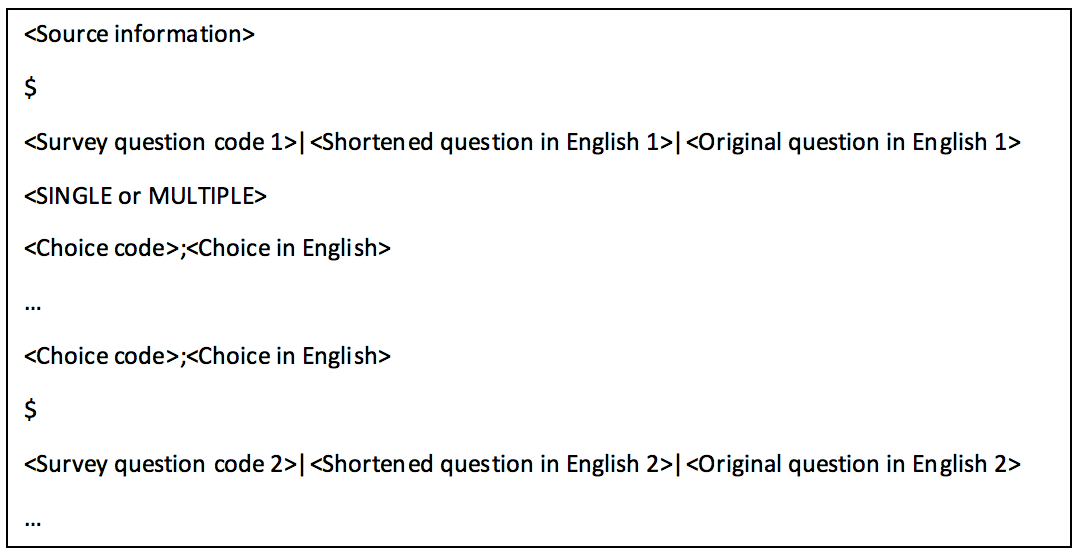
\includegraphics[scale=0.5]{textformatted}
\caption{Formatted text file of survey code translation (See Appendix for actual text)}
\end{figure}

As  seen above the text file is still readable as each question\textquotesingle s data is separated by a `\$' sign and each code is separated by a `;' or `|'. The question text is distinguishable from the choices text.

\section{System architecture}

\begin{figure}[h]
\centering
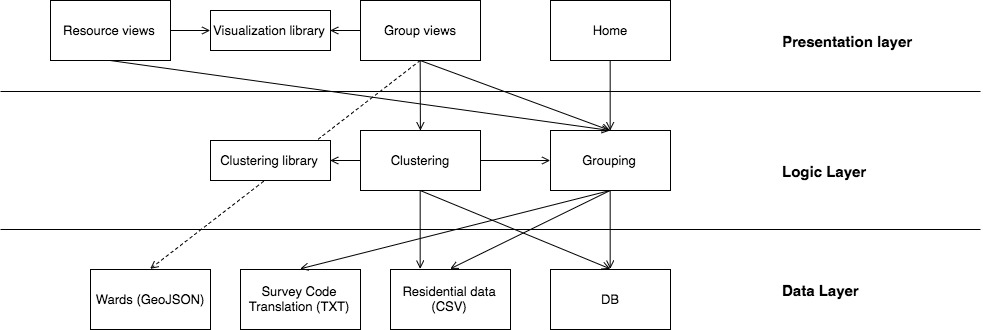
\includegraphics[scale=0.5]{FYP_Architecture}
\caption{System architecture diagram}
\end{figure}

The system will follow the three-layer architecture. \par
The data layer will consist of the following components:
\begin{itemize}
  \item \textbf{Ward}: a GeoJSON file containing the geographical boundaries of each ward
  \item \textbf{Survey Code Translation}: a text file formatted according to section \ref{preprocessing} containing the translations of the survey code to English text
  \item \textbf{Residential data}: a CSV file of the 2016 Lambeth Residential Survey
  \item \textbf{DB}: the database which includes Groups created by the user and groups\textsc{\char13} Clusters produced by the clustering algorithms (see  Appendix for more details)
\end{itemize}

The logic layer will consist of the following components:
\begin{itemize}
  \item \textbf{Clustering library}: a third-party library used by the Clustering component to cluster group data
  \item \textbf{Clustering}: performs clustering on a group and stores results in the database
  \item \textbf{Grouping}: creates groups and extracts groups from survey data
\end{itemize}

The presentation layer will consist of the following components (see section \ref{interface} for more details):
\begin{itemize}
  \item \textbf{Resource views}: shows visualizations data on each group for each question in the residential data set
  \item \textbf{Visualization library}: a third-party library used to create graph and map visualizations
  \item \textbf{Group views}: shows visualizations of groups and compares groups
  \item \textbf{Home}: main menu to choose which group to view
\end{itemize}

Though the original source of the Wards GeoJSON is from Lambeth\textquotesingle s open data website, it will be downloaded as a JSON file and stored as part of the source code of the application. Since the ward boundaries is unlikely to changing, storing the file in the source code is preferable as it will not depend on another server\textquotesingle s performance.\par

The Clustering component could be implemented separately and another clustering algorithm can be implemented without changing the Grouping component. 



\section{Algorithms}
Data analysis will be carried out by the system through data clustering. The clusters will be generated by the Clustering component and will be saved to the database. The default number of clusters is 1 and the user will be able to manipulate the number of clusters. \par

There are numerous clustering algorithms however, due to the categorical nature of the data, k-modes clustering will be used instead of the the usual k-means clustering. K-modes has been proven to be more effective in clustering categorical data (citation).

\section{User interface} \label{interface}
The system\textquotesingle s main goal is to present data and let the user interact with the user in an effective way. The following figures describe the interaction and design of the user interfaces.

\begin{figure}[h]
\centering
\includegraphics[scale=0.5]{FYP_InteractionDiagram.png}
\caption{Interaction diagram of the web application}
\end{figure}

The interaction diagram above describes the flow between the pages in the website. It is designed so that switching pages is done in the least number of clicks possible. This will be done through a navigation bar where most pages will be accessible. The group detail pages will only be accessible from the group\_detail.html page to avoid confusion with other groups\textsc{\char13} pages.\par

The following describes the functions of each page:
\begin{itemize}
  \item \textbf{index.html}: contains a list of links to all groups
  \item \textbf{group\_detail.html}: has visualizations of a group\textquotesingle s data through maps and charts (see section for more detail)
  \item \textbf{group\_compare.html}: compares all the groups to the average of the whole population of a data variable. This will visualize the comparison of the values of the cluster to the average value for that variable in the whole population (see section for more detail)
  \item \textbf{cluster\_compare.html}: compares the data on the clusters of a group, to the group and the whole population for each question (see section for more detail)
  \item \textbf{cluster\_stats.html}: lets the user change the number of clusters and shows differences, namely the means of an answer to a question, between each cluster (see section for more detail)
  \item \textbf{group\_new.html}: contains a form that adds a new group to the database
  \item \textbf{resources\_list.html}: lists links to residential survey questions
  \item \textbf{resources\_datafields.html}: shows visualizations of data on all groups for a survey question
\end{itemize}

*Note that variable is to denote the selected question and choice (i.e. Q11, Full-time employee) \par

This design gives the user different perspectives on a population. Namely, a group\textquotesingle s data (group\_detail.html), data of clusters within a group (cluster\_detail.html), differences between a group and its clusters (cluster\_compare.html, cluster\_stats.html) and differences between groups (resources\_datafields.html). These features are intended to enable the user to identify interesting trends within a specific group, groups or cluster which may not be possible with fewer interfaces. 

\section{Interface design}
The pages in the interaction diagram are described in more detail in the following page designs. Since a large part of the system is about the presentation of data, the layout of the visualizations and interactions within pages, shown as annotations, were designed.

\begin{figure}[h]
\centering
\includegraphics[scale=0.3]{FYP_Screenshots1.png}
\caption{Page design for group\_detail.html and cluster\_compare.html}
\label{fig:FYP_Screenshots1}
\end{figure}

The page on figure \ref{fig:FYP_Screenshots1} is intended for the user to view the residential data which is visualized in graphs on the right-hand side of the page. Selecting a variable (i.e. a survey question and choice) on a graph will show its data on the map, on the left-hand side of the page, as a population density map. Each ward will be colored depending on the number of residents for which the resident chose the variable. This shows the user where residents who have chosen the variable live. Supporting the map is a bar chart of the number of residents for each ward who have chosen the variable which is ordered from greatest to least. This lets the user easily identify the distribution of the selected variable throughout the wards. The charts will follow functional requirements 3, which specifies which type of graph (e.g. bar chart, pie chart, etc.) to use for which type of question.\par

In addition, the meta-data about the data set used in the page is shown in the top left panel, which shows the number of residents in the group as a raw number and percentage and the source of the data.

\begin{figure}[h]
\centering
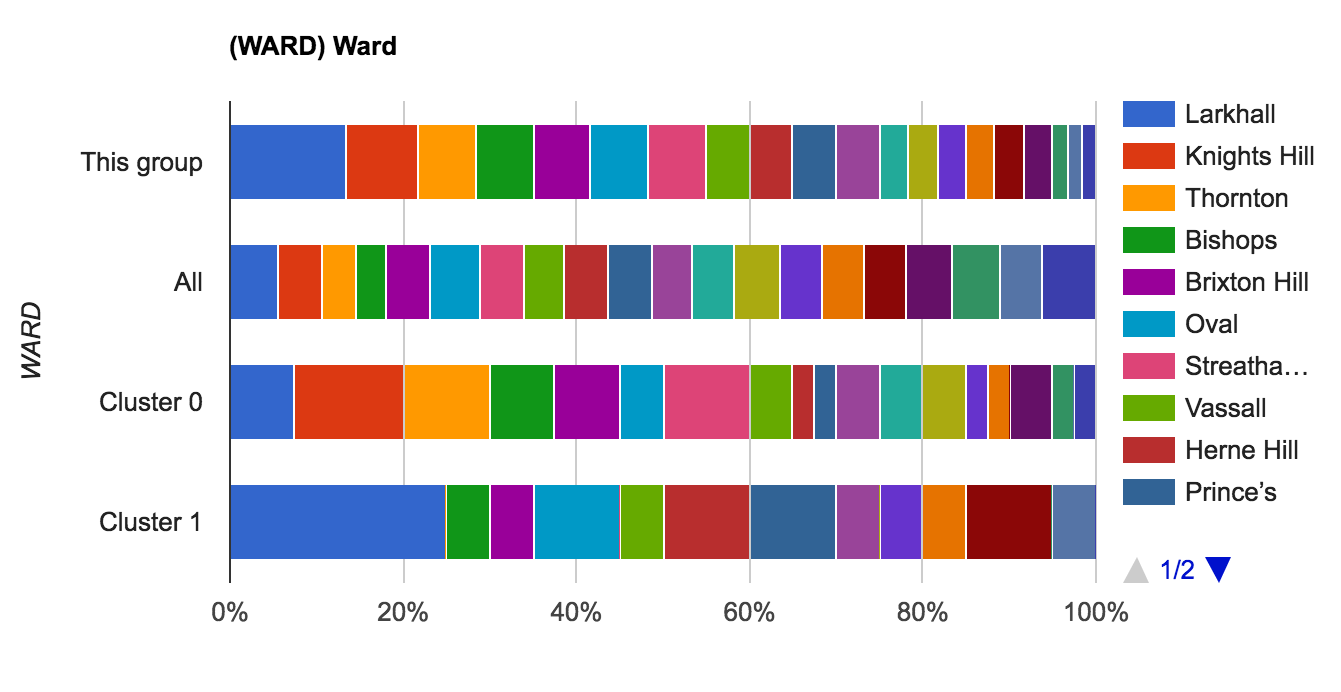
\includegraphics[scale=0.5]{comparison}
\caption{Chart for comparison of the data of the whole population, a group and its clusters}
\label{fig:comparison}
\end{figure}

The same page design is used for cluster\_compare.html except that the Question graphs will be in the form of stacked bar charts which show the question data on the whole population, the group and the clusters (see figure \ref{fig:comparison}). \par

The figure \ref{fig:comparison} is the visualization for the resources\_datafields.html page. However, the y-axis will instead be the groups in the database.

\begin{figure}[h]
\centering
\includegraphics[scale=0.3]{FYP_Screenshots2}
\caption{Page design for group\_compare.html}
\label{fig:FYP_Screenshots2}
\end{figure}

The page on figure \ref{fig:FYP_Screenshots2} will let the user compare the percent difference from the whole population using the following equation:\par

(Percent of the group\textquotesingle s population who answered selected question with selected choice-Percent of the overall population who answered selected question with selected choice)*100\par

Therefore groups more than 0\% has a bigger proportion of their population which have answered the selected variable and vice versa for groups less than 0\%. This may be an interesting visualization for some questions more than others.

\begin{figure}[h]
\centering
\includegraphics[scale=0.3]{FYP_Screenshots3}
\caption{Page design for cluster\_stats.html}
\label{fig:FYP_Screenshots3}
\end{figure}

The page on figure \ref{fig:FYP_Screenshots3} gives another perspective to the comparisons show in cluster\_compare.html. Instead of showing the all the data variables, the set of answers are consolidated into a mean. The user can compare means of a question for each cluster which will highlight the differences between each cluster which is not always obvious in cluster\_compare.html. The user may go back to cluster\_compare.html to the data in more detail.

\chapter{Implementation}

\section{Section Heading}

\chapter{Professional and Ethical Issues} \label{ch:professionalissues}

The piece of software produced is a combination of my work and the work of Third Parties, which include Open Source libraries such as Django (citation), Graphos (citation), Google Maps (citation), Google Charts (citation), Kmodes (citation), and others (citation). These libraries were utilized to take advantage of existing work however, they were adapted to the purposes of this project. Relevant libraries and sources are cited in both source code and the description in the implementation to give credit to third party content.
The main data used, the 2016 Lambeth Residential Survey, keeps its participants anonymous and according Lambeth has no security issues in terms of publicizing the data. The software places a resident under an anonymous serial, no name of any sort is saved nor a specific address. The software maintains the anonymity of the location of their residence at the Ward level instead of a more specific post code level.\par

The clustering of the survey data used a third-party software. Though sensitive information such as race and sex is included as variables in which to cluster, as far as I know the clustering algorithm used do not discriminate on those variables. \par

During the evaluation stage, a demonstration of the software was conducted to a group of 4 people from the policy department Lambeth Council to gain their feedback. The demonstration and the acceptance of their feedback was done respectfully as they have given honest criticisms of my work. \par

\chapter{Evaluation} \label{ch:evaluation}

The evaluation of the software involved the comparison between the design to the implementation. Since it is a visualization project, an independent evaluation was taken from a demonstration to some of the potential users from the policy department in Lambeth Council. The method and results of the evaluation is described below.

\section{Demonstration to Lambeth Council}

The demonstration took place in the offices of Lambeth where I presented each page of the web application. The potential of the visualization to aid the formation of strategies were discussed as well as the limitations and improvements of each feature. The requirements were given to them to compare to the actual software as well. The limitations are described below and the solutions to these limitations are in section … of the Conclusion chapter.\par

They have expressed that it has met the objectives overall and that it has the potential given that there would be more features and an option to include data sets to name a few.

The subsections below summarizes the discussions for the visualization pages and the data used.

\subsection{Data used}
The project focuses on a prototype to explore the possibilities of visualizing a population rather than creating a complete tool with usable data. The current survey data could be used as it is to facilitate the initial analysis of the population though the visualization should be taken with caution. \par

They have expressed that the usefulness of the tool relies on the quality and amount of data used. The tool may not be usable at its current state since the survey data is not representative. The current data set used only surveyed 1024 residents of a council of more than 300,000 residents. It is also uses data from only 1 year. The software does not let the user change which annual residential survey to view nor does it utilize past residential surveys.

\subsection{Group\_detail page}
This page gave much information as it not only gave data for each question, but also displaying a piece of data on the map showed where those residents live. This may help in identifying areas which need the most help.\par

In terms of the usefulness of the map, dividing it into wards limits the targeting of a smaller area since wards occupy a large area. Generalizing a ward to behave a certain way may ignore the minorities within the area. Using a smaller geographical division such as the Office of National Statistics\textsc{\char13} (ONS) output area or super output area which cover areas smaller than a ward and is included in the current data can identify more specific areas. \par

Due to the smaller data set, should there only be one resident in a ward with a given survey question, the identification of a more specific area, such as ONS\textsc{\char13} output area, would enable the user to identify if the user. For example, a ward with 1 resident in the disabled group could potentially be a person living in a senior home. This could give insights to people living in senior homes rather than a valid representation of disabled people in that ward.\par

The map\textsc{\char13}s color range was misunderstood as red meant danger and green meant good. The choice of colors could have been constrained to shades of one color.\par

\subsection{Group\_compare page}

This page gave a good indication on which questions are more applicable for which group. For example, the visualization shows more people in long-term illness and acquires child benefits are more likely to say they are not paid the London Living Wage. This could potentially help in identifying which resources should be given to which groups of people.\par

The information is limited to the percentage of a piece of data in relation to the data of a question. The comparison between groups and clusters are also in the form of percentages. Other statistical data such as mean, mode, median and standard deviation could be integrated which results in deeper analysis.

\subsection{Clusters pages}

Clustering in a statistical sense, needs to be explained to the users. Upon demonstrating the tool to the council workers, the concept of clustering needed to be explained. The visualization of the clusters as seen in cluster\_detail or cluster\_compare could only be understood given that clustering.
The cluster\_stats page was confusing as the table of means were still in the survey code. There needed to be English translations of the code supplemented. This was fixed after the demonstration where hovering over the question will show the English translations.

\subsection{Resource\_datafield page}
They were interested in this page as it has the potential to confirm or debunk some of their expectations of some groups. For example it confirmed that the ethnicities of people living in residential homes were from English, Caribbean or African descent. Another application could be how they would approach some of the groups using the questions regarding the medium of contact with the council or how they access the internet.

\section{Project evaluation}

Though the tool was inspired by the problems faced by a council based on the interview with a Lambeth council worker, the requirements and design of the tool was up to me through research into other visualization applications. Therefore, the end tool may not be suitable for them. However, they did express that it has met the requirements I have set for the software. Regular contact during the whole process in terms of feedback of the design and usability, and more specific data sets would have produced a more usable product for their needs.\par

In terms of scalability, where the data set may be more than 1042 rows, the use of Pandas Dataframe may not be suitable as it could run into performance issues. Using a database should have been used to prevent this.

\chapter{Conclusion and Future Work}

The project's conclusions should list the key things that have been learnt as a consequence of engaging in your project work. For example, ``The use of overloading in C++ provides a very elegant mechanism for transparent parallelisation of sequential programs'', or ``The overheads of linear-time n-body algorithms makes them computationally less efficient than $O(n \log n)$ algorithms for systems with less than 100000 particles''. Avoid tedious personal reflections like ``I learned a lot about C++ programming...'', or ``Simulating colliding galaxies can be real fun...''. It is common to finish the report by listing ways in which the project can be taken further. This might, for example, be a plan for turning a piece of software or hardware into a marketable product, or a set of ideas for possibly turning your project into an MPhil or PhD.

%%%%%%%%%%%%%%%%%%%%%%%%%%%%%%%%%
% References
%%%%%%%%%%%%%%%%%%%%%%%%%%%%%%%%%
\bibliographystyle{plain}
\bibliography{references}
\addcontentsline{toc}{section}{Bibliography}

%%%%%%%%%%%%%%%%%%%%%%%%%%%%%%%%%
% Appendices
%%%%%%%%%%%%%%%%%%%%%%%%%%%%%%%%%
\appendix
\include{Appendices/appendix}
\chapter{User Guide}
\section{Instructions}
You must provide an adequate user guide for your software. The guide should provide easily understood instructions on how to use your software. A particularly useful approach is to treat the user guide as a walk-through of a typical session, or set of sessions, which collectively display all of the features of your package. Technical details of how the package works are rarely required. Keep the guide concise and simple. The extensive use of diagrams, illustrating the package in action, can often be particularly helpful. The user guide is sometimes included as a chapter in the main body of the report, but is often better included in an appendix to the main report.

\chapter{Source Code}

The following pages are the Table of Contents for the source code listings and the source code themselves.
\end{document}
